
In this section, we discuss relational operators, logical operators and loop structures in Matlab.

\section{Matlab: Relational Operators}\label{sec:Matlab_relational}

If we want to compare two values, we have the following relation operations:\\
\\
\cour{< , <= , >�, >=, ==, $\sim$=}\\

It is helpful to read any statement involving these symbols as a question as the answer is either \cour{0} (false) or \cour{1} (true).\\

\index{Matlab!Relational Operators}
\example{ex_basicrelation}{{\bf Basic Relations}\\
\\
\cour{>> 3 == 4} \quad (``is 3 equal to 4?'') gives \cour{0} (false)\\
\cour{>> 3 <= 4} \quad (``is 3 less than or equal to 4?'') gives \cour{1} (true)
}

\section{Matlab: Logical Operators}\label{sec:Matlab_logical}

\index{Matlab!Logical Operators}
To create compound statments of the relational operators, we can combine these using the logical operators.  The truth or falsity of these follows basic rules of logic, so it helps to have some knowledge of truth tables. Again, read them as questions!
\begin{align*}
\cour{\&} & \qquad	\text{(``and'' returns true if both parts are true)}\\
\cour{$\sim$} & \qquad	\text{(``not'' returns true if the initial value is false)}\\
\cour{$|$} & \qquad \text{(`or'' returns true if either part is true)}\\
\cour{xor}	& \qquad \text{(``exclusive or'' returns true if either part is true, but NOT both true)}
\end{align*}



\example{ex_basiclogic}{{\bf Basic Logic}\\
\\
\cour{>> (3 >= 2) \& (3+4 == 6)}\\
\\
\cour{ans=}\\
\cour{\ps 0}

Here, the question ``is 3 greater than or equal to 2 AND 3 plus 4 equal to 6?'' is answered as false (or a zero) since even though 3 is greater than 2, it is not true that 3 plus 4 is 6.
}\\

Note that there are also the operators \&\& and $||$ which also mean ``and'' and ``or'' but are called ``short-circuited'' operators (look it up).  
As you work with these in the Editor, orange lines on the right side of the screen may appear suggesting you use \&\& in place of \& (or vice-versa) and $||$ in place of $|$ (or vice versa).  Just take those suggestions and you'll be fine.\\

These operations extend to matrices with an entry-by-entry comparison of matrices of the same size.\\

\example{ex_logic1}{\po\\
\\
\cour{>> a=[0,1;1,2], b=[0,0;1,1]}\\
\\
\cour{a =}\\
\cour{\ps 0     1}\\
\cour{\ps 1     2}\\
\cour{b =}\\
\cour{\ps 0     0}\\
\cour{\ps 1     1}\\
with\\
\\
\cour{>> a\&b, a$|$b, xor(a,b)}\\
\\
returns\\
\\
\cour{ans =}\\
\cour{\ps 0     0}\\
\cour{\ps 1     1}\\
\\
\cour{ans =}\\
\cour{\ps 0     1}\\
\cour{\ps 1     1}\\
\\
\cour{ans =}\\
\cour{\ps 0     1}\\
\cour{\ps 0     0}
}\\

One minor point to note is that while Matlab treats \cour{0} as false, any other positive whole number is considered as true.  So, in this example, even though the $(2,2)$ entry of \cour{a} is a 2, it is considered as ``true'' for logical comparison.

\index{Matlab Functions!\cour{if$\backslash$elseif}}
\index{Matlab Functions!\cour{switch$\backslash$case}}
\section{Matlab: \cour{if} and \cour{switch} commands}\label{sec:Matlab_if_switch}

We discuss the constructs \cour{if$\backslash$elseif$\backslash$else} and \cour{switch$\backslash$case$\backslash$otherwise} in this section. 

Suppose we want to have part of our program run only under certain conditions. For this, we use an \cour{if$\backslash$else} structure.  The basic format of this structure is:\\
\\
\cour{{\color{blue} if}     (put condition(s) here)}\\
\cour{\ps     (put calculations here to be run if the conditions are met)}\\
\cour{{\color{blue} elseif}    (other condition(s))}\\
\cour{\ps     (calculations that will run under the new conditions)}\\
\cour{{\color{blue} ...}   (more elseif statements, if desired)}\\
\cour{\color{blue} else}\\
\cour{\ps    (calculations run if none of the previous conditions are met)}\\
\cour{{\color{blue} end}}\\

\example{ex_ifexample}{{\bf Using \cour{if}}\\

Let's write a script M-file that lets a user input a number and then displays if that number is less than 5, 
between 5 and 10 (inclusive), or greater than 10.\\
\\
\cour{number = input({\color{myred} \tq Input a number \tq});}\\
\cour{{\color{blue} if} number < 5}\\
\cour{\ps  disp({\color{myred} \tq Your number is less than 5.\tq})}\\
\cour{{\color{blue} elseif} number >=5 \&\& number <= 10}\\
\cour{\ps  disp({\color{myred} \tq Your number is between 5 and 10.\tq})}\\
\cour{\color{blue} else}\\
\cour{\ps  disp({\color{myred} \tq Your number is greater than 10.\tq})}\\
\cour{\color{blue} end}\\

Try running this program using various numbers for input.
}\\

The \cour{switch$\backslash$case} structure is similar to the \cour{if} structure, but has a few advantages.  First of all it is easier to read and second, it is better if you are comparing strings (of possibly different lengths). The basic format is:\\
\\
\cour{{\color{blue} switch}     (expression to test)}\\
\cour{\ps {\color{blue} case} (case condition)}\\
\cour{\ps \ps(output in that case)}\\
\cour{\ps {\color{blue} case} (case condition)}\\
\cour{\ps \ps (output in that case)}\\
\cour{\ps {\color{blue} ...}(more cases)}\\
\cour{\ps \color{blue} otherwise}\\
\cour{\ps \ps (do this if no cases are met)}\\
\cour{{\color{blue} end}}\\

\example{ex_switchexample}{{\bf Using \cour{switch}}\\

Let's check to see if a cadet is in his$\backslash$her first two years at VMI.\\
\\
\cour{Year ={ \color{myred} \tq second class\tq};}\\
\\
\cour{{\color{blue} switch} Year    }\\
\cour{\ps{\color{blue} case} \{{\color{myred} \tq fourth class\tq ,\tq third class\tq }\}}\\
\cour{\ps \ps  disp({\color{myred} \tq You are in the first two years.\tq })}\\
\cour{\ps{\color{blue} case} \{{\color{myred} \tq second class\tq ,\tq first class\tq }\}}\\
\cour{\ps \ps  disp({\color{myred} \tq You are in the last two years.\tq })}\\
\cour{\ps \color{blue} otherwise}\\
\cour{\ps \ps  disp({\color{myred} \tq You must be a 5th year.\tq })}\\
\cour{\color{blue} end}\\

The cases are grouped by curly brackets so that a case will be satisfied if the value of \cour{Year} is any of the values in a specific case. Once this code is executed, the \cour{switch} command will look at the value of \cour{Year} and the output should be\\

\cour{You are in the last two years.}
}\\

\section{Matlab: \cour{for} and \cour{while} Loops}\label{sec:Matlab_loops}

\index{Matlab Functions!\cour{for}}
\index{Matlab Functions!\cour{while}}
We discuss the \cour{for} and \cour{while} loops in this section.

Suppose we want to have part of our program re-run a preset number of times.  For this, we use a \cour{for} loop. The basic format of this structure is:\\
\\
\cour{{\color{blue} for}     (put counter conditions here)}\\
\cour{\ps (put calculations here)}\\
\cour{{\color{blue}end}}\\
\\

\example{ex_forexampleonsums}{{\bf Comparing \cour{for} and \cour{sum}}\\

Let's compare two methods for adding up the first five integers.  Using the \cour{sum} command we can use\\
\\
\cour{>> sum(1:5)}\\
\cour{ans =}\\
\cour{\ps 15}\\

Now, using a \cour{for} loop to create a cumulative sum:\\
\\
\cour{totalsum=0; \color{mygreen} \% initialize}\\
\cour{{\color{blue} for} i=1:5}\\
\cour{\ps totalsum=totalsum+i;}\\
\cour{{\color{blue}end}}\\
\cour{disp(totalsum)}\\
\\
The variable \cour{totalsum} will have value 15.
}\\

In example \ref{ex_forexampleonsums}, the \cour{for} loop was the long way of doing the problem (and therefore stresses the power of the \cour{sum} function), but the following example shows a more in-depth \cour{for} loop.\\

\example{ex_forexample}{{\bf Using \cour{for}}\\

Let's find the first 10 Fibonacci numbers using the recursive definition.\\
\\
\cour{\color{mygreen} \%initialize the matrix}\\
\cour{A=zeros(1,10);}\\
\cour{A(1)=0;}\\
\cour{A(2)=1;}\\
\\
\cour{{\color{blue} for}  i=3:10}\\
\cour{\ps A(i)=A(i-1)+A(i-2);}\\
\cour{{\color{blue}end}}\\
\\
\cour{disp(A)}\\

The output for this would be\\
\\
\cour{A =}\\
{\cour{\ps 0 1 1 2 3 5 8 13 21 34}}
}\\

Now, suppose want to have part of our program run until a certain condition is met, even though we may not know how many times the loop will need to run until that happens.  For this, we use a \cour{while} loop.\\

The basic format of this structure is:\\
\\
\cour{{\color{blue}while}     (put conditions for the loop to keep running)}\\
\cour{\ps (put calculations here)}\\
\cour{{\color{blue}end}}\\
\\

Let's rewrite the last example with a slight twist.  Let's find the Fibonacci numbers until they exceed 1000.\\

\example{ex_whileexample}{{\bf Using \cour{while}}\\

\noindent \cour{\color{mygreen} \%initialize the matrix (we don�t know how big it will be so}\\
\cour{\color{mygreen} \% \po \po we will grow it in the while loop).}\\
\cour{A(1)=0;}\\
\cour{A(2)=1;}\\
\cour{j=2; {\color{mygreen} \%initialize a counter}}\\
\cour{{\color{blue}while} A(j) < 1000}\\
\cour{\ps j=j+1; \color{mygreen} \%move the counter along}\\
\cour{\ps A(j)=A(j-1)+A(j-2);  }\\
\cour{{\color{blue}end}}\\
\\
\cour{disp(A)}\\

The output for this would be\\
\\
\cour{A =}\\
{\cour{\ps 0 1 1 2 3 5 8 13 21 34 55 89 144 233 377 610 987 1597}}\\

The loop concludes when we pass 1000.  
}


\newpage
\printexercises{exercises/07_exercises}

%
%
%\vspace{1in}
%EXERCISES:\\
%1) Modify your RemoveRow Function from the previous homework in two ways (you should have two different functions):\\
%a) Use an \cour{if} loop to have an error message displayed if the user enters an invalid row.  Then prompt them to enter a new row number.  In your prompt, you must indicate the allowable range of rows.  Here they only have one chance to re-enter the row.\\
%b) Use a \cour{while} loop so that if the user enters an invalid row on their first try, they will be able to continue to enter rows until they enter a correct value.  Again, in your prompt, you must indicate the allowable range of rows. 


%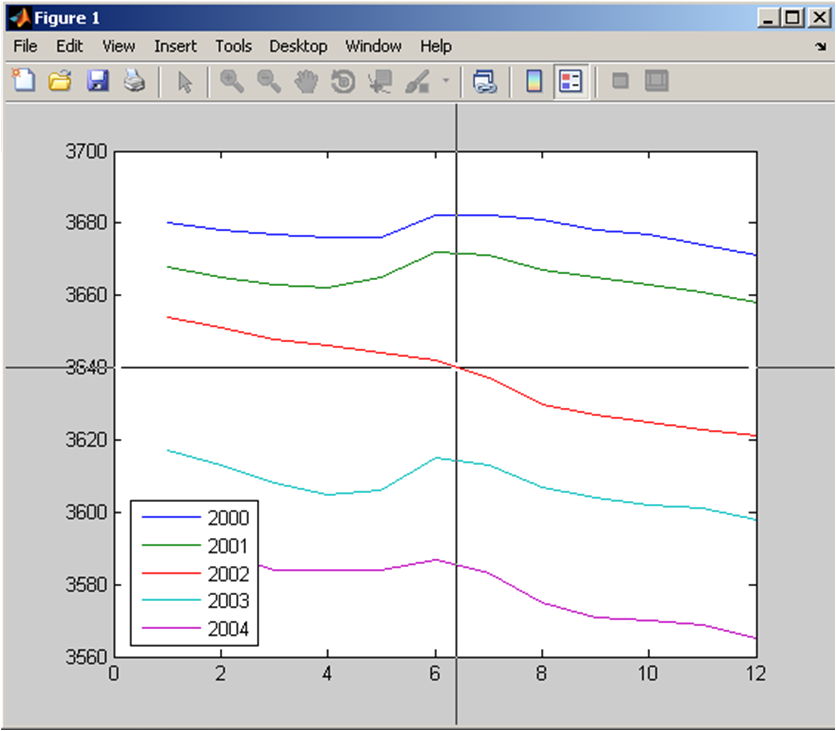
\includegraphics[scale=.75]{figures/matlab_ginput.png}

%\definition{def:lineintegral}{\textbf{TITLE}}
%
%\keyidea{idea:lineintprops}{\textbf{TITLE}}
%
%\printexercises{exercises/mathcad_introduction_exercises}
